

\subsection{Lower bound}

In the case of general trees, Gavoille et al~\cite{Gavoille200485} establish a lower bound  of $\frac{1}{8}\log^2 n-O(\log n)$ using an ingenious technique where they apply a distance labeling scheme to a special class of trees called $(h,M)$-trees\footnote{Note that their exposition has some minor errors as pointed out (and corrected) in~\cite{esbenthesis}}. The following uses a generalization of $(h,M)$-trees to improve their ideas and leads to a lower bound of $\frac{1}{4}\log^2 n-O(\log n)$.

\paragraph{$(h,W,a)$-trees.}
We begin with some definitions. For integers $h,W\geq 0$ and a number $a\geq 1$ such that $W/a^i$ is integral for all $i=0,\dots ,h$, an \emph{$(h,W,a)$-tree} is a rooted binary tree $T$ with edge weights in $[0,W]$ that is constructed recursively as follows. For $h=0$, $T$ is just a single node. For $h=1$, $T$ is a claw (i.e.\ a star with three edges) with edge weights $x,x,W-x$ for some $0\leq x<W$ rooted at the leaf node of the edge with weight $W-x$. For $h>1$, $T$ consists of an $(1,W,a)$-tree whose two leaves are the roots of two $(h-1,W/a,a)$-trees $T_0,T_1$.  We shall denote an $(h,W,a)$-tree constructed in this way by $T=\langle T_0,T_1,x\rangle$
An example for $h=3$ can be seen in \Cref{fig:hMtree}. Note that the case $a=1$ simply corresponds to the $(h,W)$-trees defined in~\cite{Gavoille200485}.

\begin{figure}
	\centering
	\begin{tikzpicture}[sibling distance=3em, inner sep=0pt, minimum size=1ex]
	\tikzstyle{every node}=[draw,circle,fill=black]
	\Tree [.{} \edge node[draw=none,fill=none,auto=right] {$W-x$}; [.{} 
		\edge node[draw=none,fill=none,auto=right] {$x$}; [.{} \edge node[draw=none,fill=none,auto=right] {$\frac{W}{a}-y_1$}; [.{} 
			\edge node[draw=none,fill=none,auto=right] {$y_1$}; [.{} \edge node[draw=none,fill=none,draw=none,fill=none,auto=right] {$\frac{W}{a^2}-z_1$}; [.{} \edge node[draw=none,fill=none,auto=right,pos=.6] {$z_1$}; [ .{} ] \edge node[draw=none,fill=none,auto=left,pos=.6] {$z_1$}; [ .{} ] ] ]
			\edge node[draw=none,fill=none,auto=left] {$y_1$}; [.{} \edge node[draw=none,fill=none,auto=left] {$\frac{W}{a^2}-z_2$}; [.{} \edge node[draw=none,fill=none,auto=right,pos=.6] {$z_2$}; [ .{} ] \edge node[draw=none,fill=none,auto=left,pos=.6] {$z_2$}; [ .{} ] ] ]
			]
		]
		\edge node[draw=none,fill=none,auto=left] {$x$}; [.{}	\edge node[draw=none,fill=none,auto=left] {$\frac{W}{a}-y_2$}; [.{}
			\edge node[draw=none,fill=none,auto=right] {$y_2$}; [.{} \edge node[draw=none,fill=none,auto=right] {$\frac{W}{a^2}-z_3$}; [.{} \edge node[draw=none,fill=none,auto=right,pos=.6] {$z_3$}; [ .{} ] \edge node[draw=none,fill=none,auto=left,pos=.6] {$z_3$}; [ .{} ] ] ]
			\edge node[draw=none,fill=none,auto=left] {$y_2$}; [.{} \edge node[draw=none,fill=none,auto=left] {$\frac{W}{a^2}-z_4$}; [.{} \edge node[draw=none,fill=none,auto=right,pos=.6] {$z_4$}; [ .{} ] \edge node[draw=none,fill=none,auto=left,pos=.6] {$z_4$}; [ .{} ] ] ] 
			] 
		] 
	] ]
	\end{tikzpicture}
	\caption{An $(h,W,a)$-tree, where $h=3$. We require that $x<W$, $y_1,y_2<W/a$ and $z_1,\dots ,z_4<W/a^2$.
}
	\label{fig:hMtree}
\end{figure}


It is easy to see that an $(h,W,a)$-tree
has $2^h$ leaves and $3\cdot 2^h-2$ nodes.  Further, it is straightforward to see that, if $u,v$ are leaves in an $(h,W,a)$-tree $T=\langle T_0,T_1,x\rangle$, then
\begin{equation} \label{eq:disthM}
\dist_T(u,v)= \begin{cases} 2W\frac{a^{-1}-a^{-h}}{1-a^{-1}} + 2x,& \text{if $u\in T_0$ and $v\in T_1$, or vice versa,} \\ \dist_{T_i}(u,v), & \text{if $u,v\in T_i$ for some $i=0,1$}.\end{cases}
\end{equation}

\paragraph{Leaf distance labeling schemes.}
In the following we shall consider \emph{leaf distance labeling schemes} for the family of $(h,W,a)$-trees: that is, distance labeling schemes where only the leaves in a tree need to be labeled, and where only leaf labels can be given as input to the decoder. Since an ordinary distance labeling scheme obviously can be used only for leaves, any lower bound on worst-case label sizes for a leaf distance labeling scheme is also a lower bound for an ordinary distance labeling scheme. We denote by $g(h,W,a)$ the smallest number of labels needed by an optimal leaf distance labeling scheme to label all $(h,W,a)$-trees.
\begin{lemma} \label{lemm:distancehM}
For all $h\geq 1$ and $W\geq 2$, $g(h,W,a)^2\geq Wg(h-1,W^2/a^2,a^2)$.
\end{lemma}
\begin{proof}
Fix an optimal leaf distance labeling scheme $\scheme$ which produces exactly $g(h,W,a)$ distinct labels for the family of $(h,W,a)$-trees. For leaves $u$ and $v$ in an $(h,W,a)$-tree, denote by $l(u)$ and $l(v)$, respectively, the labels assigned by $\scheme$. For $x=0,\dots ,W-1$, let $S(x)$ be the set consisting of pairs of labels $(l(u),l(v))$ for all leaves $u\in T_0$ and $v\in T_1$ in all $(h,W,a)$-trees $T=\langle T_0,T_1,x\rangle$.

The sets $S(x)$ and $S(x')$ are disjoint for $x\neq x'$, since every pair of labels in $S(x)$ uniquely determines $x$ due to~\eqref{eq:disthM}. Letting $S=\bigcup_{x=0}^{W-1}S(x)$, we therefore have $|S|=\sum_{x=0}^{W-1}|S(x)|$. 
Since $S$ contains pairs of labels produced by $\scheme$ from leaves in $(h,W,a)$-trees , we clearly also have $|S|\leq g(h,W,a)^2$, and hence it only remains to prove that $|S|\geq Wg(h-1,W^2/a^2,a^2)$, which we shall do by showing that $|S(x)|\geq g(h-1,W^2/a^2,a^2)$ for all $x$.

The goal for the rest of the proof is therefore to create a leaf distance labeling scheme for $(h-1,W^2/a^2,a^2)$-trees using only labels from the set $S(x)$ for some fixed $x$. So let $x$ be given and consider an $(h-1,W^2/a^2,a^2)$-tree $T'$. Let  $V=W/a$. From $T'$ we shall construct an $(h-1,V,a)$-tree $\phi_i(T')$ for $i=0,1$ such that every leaf node $v$ in $T'$ corresponds to nodes $\phi_i(v)$ in $\phi_i(T')$ for $i=0,1$.
The trees $\phi_i(T')$ are defined as follows.
If $h=1$, so that $T'$ consists of a single node, then $\phi_i(T')=T'$ for $i=0,1$. 
If $h>1$, then $T'$ is in the form $T'=\langle T'_0,T'_1,y\rangle$ for some $0\leq y< V^2$. We can write $y$ in the form $y=y_0+y_1V$ for uniquely determined $y_0,y_1$ with $0\leq y_0,y_1<V$. For $i=0,1$, we recursively define $\phi_i(T') = \langle \phi_i(T'_0), \phi_i(T'_1),y_i\rangle$. Thus, $\phi_i(T')$ is an $(h-1,V,a)$-tree that is similar to $T'$ but where we replace the top edge weight $y$ by edge weights $y_i$ and, recursively, do the same for all $(h-2,V^2/a^2,a^2)$-subtrees. Note also that the corresponding edge weight $V^2-y$ in $T'$ automatically is replaced by the edge weight $V-y_i$ in $\phi_i(T')$ in order for $\phi_i(T')$ to be an $(h-1,V,a)$-tree.

Denote by $\phi_i(v)$ the leaf in $\phi_i(T')$ corresponding to the leaf $v$ in $T'$.

Consider now the $(h,W,a)$-tree $T=\langle \phi_0(T'),\phi_1(T'),x\rangle$. Every leaf $v$ in $T'$ corresponds to the leaves $\phi_0(v),\phi_1(v)$ in $T$ where $\phi_i(v)\in \phi_i(T')$ for $i=0,1$. 
Using  formula~\eqref{eq:disthM} for the distances in $T'$, it is straightforward to see that
\begin{equation*} \label{eq:disthMdistances}
\dist_{T'}(u,v) = \left(\dist_{\phi_0(T')}(\phi_0(u),\phi_0(v)) \bmod (2V)\right) + V\dist_{\phi_1(T')}(\phi_1(u),\phi_1(v)).
\end{equation*}

We can now apply the leaf distance labeling scheme $\scheme$ to $T$ and obtain a label for each leaf node in $T$. In particular, the pair of leaves $(\phi_0(v),\phi_1(v))$ corresponding to a node $v$ in $T'$ will receive a pair of labels. We use this pair to label $v$ in $T'$, whereby we have obtained a labeling of the leaves in $T'$ with labels from $S(x)$. Using the formula in~\eqref{eq:disthMdistances} we can construct a decoder that can compute the distance between two nodes in $T'$ using these labels alone, and hence we have obtained a leaf distance labeling scheme for $(h-1,V^2,a^2)$-trees using only labels from $S(x)$ as desired.
\end{proof}

\begin{lemma} \label{lemm:distancehM2}
For all $h\geq 1$ and $W\geq 2$, $g(h,W,a)\geq \frac{W^{h/2}}{a^{h(h-1)/4}}$.
\end{lemma}
\begin{proof}
The proof is by induction on $h$. For $h=1$ we note that an $(0,W,a)$-tree has only one node, so that $g(0,W^2/a^2,a^2)=1$. \Cref{lemm:distancehM} therefore yields $g(1,W,a)^2\geq W$ from which it follows that $g(1,W,a)\geq \sqrt{W}$. The lemma therefore holds for $h=1$. Now let $h>1$ and assume that the lemma holds for $h-1$. \Cref{lemm:distancehM} and the induction hypothesis now yield
\begin{align*}
g(h,W,a)^2 &\geq Wg(h-1,W^2/a^2,a^2) \\
 & \geq W  \frac{(W^2/a^2)^{(h-1)/2}}{a^{2(h-1)(h-2)/4}}  \\
 &= \frac{W^h}{a^{h(h-1)/2}}
\end{align*}
from which it follows that $g(h,W,a)\geq  \frac{W^{h/2}}{a^{h(h-1)/4}}$ as desired.
\end{proof}

The previous lemma implies that any (leaf and hence also ordinary) distance labeling scheme for $(h,W,a)$-trees must have labels with worst-case length at least $\frac{h}{2}(\log W-\frac{h-1}{2}\log a) = \frac{1}{2}h\log W-\frac{1}{4}h^2\log a+\frac{1}{4}h\log a$. Since the number of nodes in such a tree is $n=3\cdot 2^h-2$, it follows that $h=\log (n+2)-\log 3$, and hence that $\log n-2\leq h\leq \log n$ for sufficiently large $n$. From this we see that the worst case label length is at least 
\[
\frac{1}{2}\log n\log W-\frac{1}{4}\log n (\log n - 1)\log a-\log W -\frac{1}{2}\log a.
\]
In the case where $a=1$, we retrieve the bound of $\frac{1}{2}\log n\log W-\log W$ obtained in~\cite{gavoillepelegperennesraz}. It seems that larger values of $a$ only makes the above result weaker, but the the real strength of the above becomes apparent when we switch to the unweighted version of $(h,W,a)$-trees, in which we replace weighted edges by paths of similar lenghts. Note that a distance labeling scheme for the family of unweighted $(h,W,a)$-trees can be used as a distance labeling scheme for the weighted $(h,W,a)$-trees, and hence any lower bound in the weighted version automatcially becomes a lower bound in the unweighted version.

The number of nodes $n$ in an \emph{unweighted} $(h,W,a)$-tree is upper bounded by
\[
n\leq  2W+2\cdot 2W/a + 2^2\cdot 2W/a^2 + \dots + 2^{h-1}\cdot 2W/a^{h-1} +1
\]
In the case $a=2$, we get $n \leq 2Wh+1$.

\begin{theorem} \label{theo:distancelowerbintrees}
Any distance labeling scheme for unweighted $(h,W,2)$-trees, and hence also for general trees, has a worst-case label size of at least $\frac{1}{4}\log^2 n-O(\log n)$.
\end{theorem}
\begin{proof}
Choose the largest integer $h$ with $2\cdot 2^hh+1\leq n$, and note that we must have $h\geq \log n-O(\log\log n)$.  Set $W=2^h$ and consider the family of  $(h,W,2)$-trees, which is a subfamily of the family of trees with $n$ nodes. From \Cref{lemm:distancehM2} it therefore follows that the worst-case label length is
\begin{align*}
\frac{1}{2}h\log W-\frac{1}{4}h^2+\frac{1}{4}h &= \frac{1}{4}h^2 +\frac{1}{4}h 
 = \frac{1}{4}\log^2 n + \frac{1}{4}\log n -O(\log\log  n). \qedhere
\end{align*}
\end{proof}
